\documentclass[11pt]{article}

%% MinionPro fonts 
%\usepackage[lf]{MinionPro}
%\usepackage{MnSymbol}
\usepackage{microtype}

%% Margins
\usepackage{geometry}
\geometry{verbose,letterpaper,tmargin=1in,bmargin=1in,lmargin=1in,rmargin=1in}

%% Other packages
\usepackage{amssymb}
\usepackage{amsmath}
\usepackage{amsthm}
\usepackage[shortlabels]{enumitem}
\usepackage{titlesec}
\usepackage{soul}
\usepackage{tikz}
\usepackage{mathtools}
\usepackage{pgfplots}
\usepackage{tikz-3dplot}
\usepackage{algorithmic}
\usepackage[export]{adjustbox}
\usepackage{tcolorbox}

%% Paragraph style settings
\setlength{\parskip}{\medskipamount}
\setlength{\parindent}{0pt}

%% Change itemize bullets
\renewcommand{\labelitemi}{$\bullet$}
\renewcommand{\labelitemii}{$\circ$}
\renewcommand{\labelitemiii}{$\diamond$}
\renewcommand{\labelitemiv}{$\cdot$}

%% Colors
\definecolor{rred}{RGB}{204,0,0}
\definecolor{ggreen}{RGB}{0,145,0}
\definecolor{yyellow}{RGB}{255,185,0}
\definecolor{bblue}{rgb}{0.2,0.2,0.7}
\definecolor{ggray}{RGB}{190,190,190}
\definecolor{ppurple}{RGB}{160,32,240}
\definecolor{oorange}{RGB}{255,165,0}

%% Shrink section fonts
\titleformat*{\section}{\normalsize\bf}
\titleformat*{\subsection}{\normalsize\bf}
\titleformat*{\subsubsection}{\normalsize\it}

% %% Compress the spacing around section titles
\titlespacing*{\section}{0pt}{1.5ex}{0.75ex}
\titlespacing*{\subsection}{0pt}{1ex}{0.5ex}
\titlespacing*{\subsubsection}{0pt}{1ex}{0.5ex}

%% amsthm settings
\theoremstyle{definition}
\newtheorem{problem}{Problem}
\newtheorem{example}{Example}
\newtheorem*{theorem}{Theorem}
\newtheorem*{bigthm}{Big Theorem}
\newtheorem*{biggerthm}{Bigger Theorem}
\newtheorem*{bigcor1}{Big Corollary 1}
\newtheorem*{bigcor2}{Big Corollary 2}

%% tikz settings
\usetikzlibrary{calc}
\usetikzlibrary{patterns}
\usetikzlibrary{decorations}
\usepgfplotslibrary{polar}

%% algorithmic setup
\algsetup{linenodelimiter=}
\renewcommand{\algorithmiccomment}[1]{\quad// #1}
\renewcommand{\algorithmicrequire}{\emph{Input:}}
\renewcommand{\algorithmicensure}{\emph{Output:}}

%% Answer box macros
%% \answerbox{alignment}{width}{height}
\newcommand{\answerbox}[3]{%
  \fbox{%
    \begin{minipage}[#1]{#2}
      \hfill\vspace{#3}
    \end{minipage}
  }
}

%% \answerboxfull{alignment}{height}
\newcommand{\answerboxfull}[2]{%
  \answerbox{#1}{6.38in}{#2} 
}

%% \answerboxone{alignment}{height} -- for first-level bullet
\newcommand{\answerboxone}[2]{%
  \answerbox{#1}{6.0in}{#2} 
}

%% \answerboxtwo{alignment}{height} -- for second-level bullet
\newcommand{\answerboxtwo}[2]{%
  \answerbox{#1}{5.8in}{#2}
}

%% special boxes
\newcommand{\wordbox}{\answerbox{c}{1.2in}{.5cm}}
\newcommand{\catbox}{\answerbox{c}{.5in}{.7cm}}
\newcommand{\letterbox}{\answerbox{c}{.7cm}{.5cm}}

%% Miscellaneous macros
\newcommand{\tstack}[1]{\begin{multlined}[t] #1 \end{multlined}}
\newcommand{\cstack}[1]{\begin{multlined}[c] #1 \end{multlined}}
\newcommand{\ccite}[1]{\only<presentation>{{\scriptsize\color{gray} #1}}\only<article>{{\small [#1]}}}
\newcommand{\grad}{\nabla}
\newcommand{\ra}{\ensuremath{\rightarrow}~}
\newcommand{\maximize}{\text{maximize}}
\newcommand{\minimize}{\text{minimize}}
\newcommand{\subjectto}{\text{subject to}}
\newcommand{\trans}{\mathsf{T}}
\newcommand{\bb}{\mathbf{b}}
\newcommand{\bx}{\mathbf{x}}
\newcommand{\bc}{\mathbf{c}}
\newcommand{\bd}{\mathbf{d}}

%% LP format
%    \begin{align*}
%      \maximize \quad & \mathbf{c}^{\trans} \mathbf{x}\\
%      \subjectto \quad & A \mathbf{x} = \mathbf{b}\\
%                       & \mathbf{x} \ge \mathbf{0}
%    \end{align*}


%% Redefine maketitle
\makeatletter
\renewcommand{\maketitle}{
  \noindent SA405 -- AMP \hfill Rader \S 3.1 \\

  \begin{center}\Large{\textbf{\@title}}\end{center}
}
\makeatother

%% ----- Begin document ----- %%
\begin{document}
  
\title{Lesson 6.  Introduction to Binary Variables}

\maketitle

%%%
\section{Today...}

\begin{itemize}
	\item  We extend a min-cost network flow model to a \emph{fixed-charge facility location} model.
	\item  This will require the use of \emph{binary decision variables}.
	\item  There are two well-known formulations for modeling the fixed-charge forcing constraints:  the so-called \emph{weak} and \emph{strong} formulations.
\end{itemize}

\section{Cloud Nine Department Store}
Cloud Nine is considering 3 locations for new distribution centers to serve its customers in 4 nearby cities.  The following table shows the fixed cost (in millions of dollars) of opening each potential center, the number (in thousands) of truckloads forecasted to be demanded at each city over the next 5 years, and the transporation cost (in millions of dollars) per thousand truckloads moved from each center location to each city.  

\begin{center}
\begin{tabular}{c|c|cccc}
& Fixed & \multicolumn{4}{c}{Transport Costs} \\
& Cost & City 1 & City 2 & City 3 & City 4\\
\hline
Distribution center 1 & 200 & 6 & 5 & 9 & 3  \\
Distribution center 2 & 400 & 4 & 3 & 5 & 6 \\
Distribution center 3 & 225 & 5 & 8 & 2 & 4 \\
\hline
Demand & --- & 11 & 18 & 15 & 25
\end{tabular}
\end{center}

Cloud Nine seeks a minimum cost distribution system assuming any distribution center can meet any or all demands.

\begin{center}
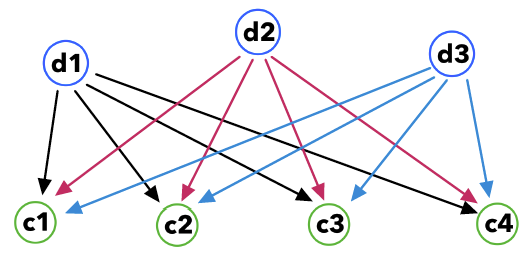
\includegraphics[width=.7\textwidth]{network}
\end{center}

\newpage
\section{Concrete transportation model, ignoring fixed cost for opening centers}
\begin{problem}
\emph{Ignoring the facility opening costs}, write a concrete model (objective function and constraints only) for this transportation problem.  Let $x_{ij}$ represent the number of truckloads to move from center 
$i$ to city $j$, and assume that each center is capable of supplying enough truckloads to meet all demand.
\end{problem}

\answerboxfull{c}{2.8in}

%%%
\bigskip
\section{Binary Decision Variables for Distribution Centers}

The use of binary $\{0,1\}$ variables to model yes/no decisions is very common.  In this model, we use a binary decision variable for each potential distribution center (DC) that indicates whether or not it is used in the solution:


\[ 
z_1 = \begin{cases}  1 \text{~~if DC 1 is opened} \\ 0 \text{~~if DC 1 is not opened}\end{cases} 
z_2 = \begin{cases}  1 \text{~~if DC 2 is opened} \\ 0 \text{~~if DC 2 is not opened}\end{cases} 
z_3 = \begin{cases}  1 \text{~~if DC 3 is opened} \\ 0 \text{~~if DC 3 is not opened}\end{cases} 
\] 

\bigskip
\section{Objective function with fixed costs}
\begin{problem}
Modify the concrete objective function in the model above to incorporate the fixed costs to open distribution centers.
\end{problem}
\answerboxfull{c}{1.7in}

\newpage

\section{Fixed-charge constraints}

\begin{itemize}
\item Whenever we use binary decision variables, we must include constraints that enforce the correct behavior of the variables in the context of the model.  
%\item This can require some thought, careful logic, and even creativity.  
\item In this problem, we need constraints that enforce the logic: \textbf{If a DC is closed, then we can't ship out of that DC.}
\item Without this logic, we wouldn't be forced to pay the fixed cost to open a warehouse.
\item There are two options for fixed-charge constraints:  ``single-variable''  \textbf{OR} ``multiple-variable''. 
\end{itemize}

\begin{problem}  (\emph{``Single-variable'' fixed-charge constraints}) 

\vspace{-.1in}
\begin{enumerate}[a.]
\item Write an inequality that enforces the logic:
\textbf{ If $z_1 = 0$, then $x_{11} = 0$.}  Include a coefficient on  $z_1$ so that the constraint allows $x_{11}$ to be large enough to ship all of the demand required by city 1 out of d.c. 1 if $z_1=1$ (DC 1 is open).

\answerboxone{c}{0.5 in}

\item[] \textbf{These are often referred to as \emph{strong} constraints.}
\item Write all of the ``strong'' fixed-charge constraints required in the concrete model.

\answerboxone{c}{1.5 in}
\end{enumerate}
\end{problem}

\newpage
\begin{problem} (\emph{``Multiple-variable'' fixed-charge constraints})

\vspace{-.1in}
\begin{enumerate}[a.]
\item Write an inequality that enforces the logic: \textbf{If $z_1 = 0$, then $x_{11} = x_{12} = x_{13} = 0$.}  Include a coefficient on $z_1$ to allow $x_{11}, x_{12}$, and  $x_{13}$ to be large enough to ship all of the demand out of d.c. 1 if $z_1=1$ (DC 1 is open). \\ \answerboxone{c}{0.5 in}

\item[] \textbf{These are often referred to ask \emph{weak} constraints.}

\item Write all of the ``weak'' fixed-charge constraints required in the concrete model. \\  \answerboxone{c}{1.5 in}

\end{enumerate}
\end{problem}

\newpage

%%%
\newpage
\section{Parameterized Model: Fixed-Charge Facility Location}

The basic min-cost (transportation) network flow portion of the model is provided below.  Extend this model to incorporate the facility location opening fee, or the ``fixed charge''.  The new collection of variables are \textbf{binary $\{0,1\}$ decision variables}.  

\textbf{Sets:}

		\begin{tabular}{ll}
			$D := $ & the set of distribution centers \\
			$C := $ & the set of cities \\
		\end{tabular}

\textbf{Parameters:}
		
		\begin{tabular}{rl}
			$c_{ij} := $ & the cost (in millions) to deliver 1000 truckloads from center $i$ to city $j$,  \\
			& for $i \in D$ and $j \in C$ \\
			$d_j := $ & the demand (in thousands) of truckloads forecasted for city $j$, for $j \in C$ \\
			$f_i  :=$ & \answerbox{c}{5.5in}{0.7cm} \\
			$M :=$ & \answerbox{c}{5.5in}{0.7cm}
		\end{tabular}

\textbf{Decision Variables:}
		
		\begin{tabular}{rl}
			$x_{ij} := $ & the number (in thousands) of \textbf{whole} truckloads to deliver from center $i$ to  city $j$, \\
			& for $i \in D$ and $j \in C$ \\
			$z_i :=$ & \answerbox{c}{5.5in}{0.7cm}
		\end{tabular}
		
\bigskip	
\textbf{Model:}  \emph{(Add comments to describe the objective function and each constraint.)}
		
    \begin{flalign*}
      \maximize \quad & \sum_{i \in D} \sum_{j \in C} c_{ij} x_{ij} + \answerbox{c}{2in}{1cm} &\\
      \\
      \subjectto \quad & \sum_{i \in D} x_{ij} \geq d_j, \text{ for all } j \in C  &\\
			  & \text{\emph{strong fixed-charge constraints:} } & \\
      			  & \answerbox{c}{3in}{1cm} &\\
			 & \text{~~~~~OR} & \\
			  & \text{\emph{weak fixed-charge constraints:} } & \\
      			  & \answerbox{c}{3in}{1cm} &\\ \\		 
                       & x_{i,j} \in \mathbb{Z}^{\geq 0}, \text{for all } i \in D, j \in C \text{~~~~~~(We don't get integer solutions for free! Why not?)}&\\ 
			  & \answerbox{c}{2in}{1cm} & \\
    \end{flalign*}
	


		


\end{document}
